% This text is proprietary.
% It's a part of presentation made by myself.
% It may not used commercial.
% The noncommercial use such as private and study is free
% Nov. 2006
% Author: Sascha Frank 
% University Freiburg 
% www.informatik.uni-freiburg.de/~frank/
%
% additional usepackage{beamerthemeshadow} is used
%  
%  \beamersetuncovermixins{\opaqueness<1>{25}}{\opaqueness<2->{15}}
%  with this the elements which were coming soon were only hinted
\documentclass{beamer}
%\usepackage{beamerthemesplit}
\usepackage{asymptote}
\usepackage[update,prepend]{epstopdf}
\usepackage{subfigure}
%\usepackage{cite}
%\usepackage[cmex10]{amsmath}
\usepackage{amsfonts}
\usepackage{url}
\usepackage{pgf}
\usepackage{tikz}
\usetikzlibrary{arrows,chains,matrix,positioning,scopes}
%
\makeatletter
\tikzset{join/.code=\tikzset{after node path={%
\ifx\tikzchainprevious\pgfutil@empty\else(\tikzchainprevious)%
edge[every join]#1(\tikzchaincurrent)\fi}}}
\makeatother
%
\tikzset{>=stealth',every on chain/.append style={join},
         every join/.style={->}}
\tikzstyle{labeled}=[execute at begin node=$\scriptstyle,
   execute at end node=$]
\usepackage[style=ieee]{biblatex}
\addbibresource{presentation}
%\ExecuteBibliographyOptions{numeric-comp}
\usepackage{wrapfig}
\def\docversion{Notes Version 0.1}

\usetheme{Luebeck}
\usecolortheme{lily}
\usefonttheme{serif}
\title{Sensors for FRC}  
\author{Dr. Travis W. Axtell \\ \emph{travis.axtell@gmail.com}}
\institute{Mentor for FRC Team 612 --- Chantilly, VA \\ 
\quad\quad\quad\, FRC Team 
2035 --- 
Carmel, CA \\ \quad\quad\quad\quad\quad\quad FRC Team 5104 --- Pacific Grove, 
CA}
\date{\docversion\\ \today} 

\addtobeamertemplate{footnote}{}{\vspace{2ex}}

\setbeamercolor{block title}{use=structure,fg=white,bg=blue!75!black}
\setbeamercolor{block body}{use=structure,fg=black,bg=black!20!white}
\setbeamertemplate{blocks}[rounded][shadow=true]
%\setbeamertemplate{blocks}

\begin{document}

\frame{\titlepage} 

\frame{\frametitle{Table of contents}\tableofcontents} 


\section{Introduction} 
\frame{ 
\frametitle{How to read these notes}
\begin{itemize}
\item Underlined terms are concepts you should strive to understand, with the 
goal of being able to explain the concepts to others.
\item Investigate the meaning of new math notation.  Wikipedia can help --- see 
\url{https://en.wikipedia.org/wiki/List_of_mathematical_symbols}.
\item I am available for discussions when you need help.
\end{itemize}
}

\subsection{Robot Hardware}
\frame{
\frametitle{RobotRIO (the ``robot brain'')}
\includegraphics[width=\textwidth]{RobotRio}
}

\frame{
\frametitle{Old hardware connection options (for comparison only)}
\includegraphics[width=2.5in]{DigitalSideCar}
\includegraphics[width=2in]{AnalogSideCar}
}

\subsection{Definitions}
\frame{\frametitle{Definitions}
An \underline{input} signal is a signal generated on some external hardware 
that is going into the RobotRIO.
\\
An \underline{output} signal is a signal generated on the RobotRIO that is 
going to external hardware.
\\
A \underline{digital input/output} port (DIO) on the RobotRIO can perform 
either 
input or output, but not both.
}




\frame{\frametitle{Analog signals}
\begin{figure}
\centering
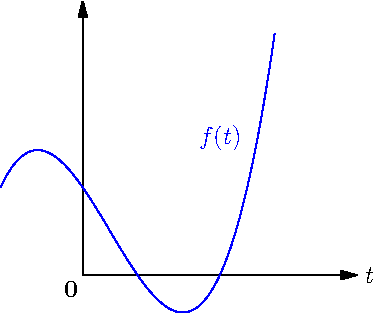
\includegraphics[width=2in]{analog}
\end{figure}
A \underline{analog signal} represents a varying quantity using a continuous 
independent variable, such as time.
\\
Examples: acoustic, acceleration, velocity, pressure, temperature --- many 
examples exist in nature.
}

\frame{\frametitle{Digital signals}
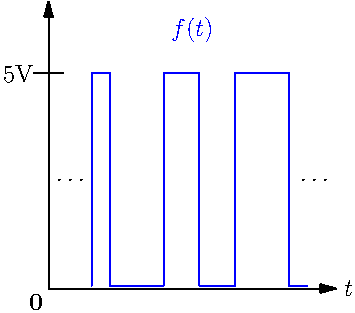
\includegraphics[width=2in]{pwm} 
\hspace{0.2cm}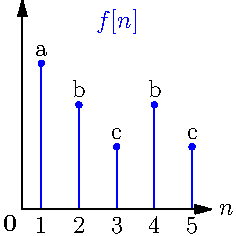
\includegraphics[width=1.75in]{digital}
\\
A \underline{digital signal} can be represented in two ways:
\begin{enumerate}
\item a continuous-time \underline{waveform} representing a bit stream 
(transitions occur at discrete times)
\item a discrete-time \underline{pulse train} of discrete values
\end{enumerate}
}

\begin{frame}[shrink]{PWM signal}
\begin{figure}
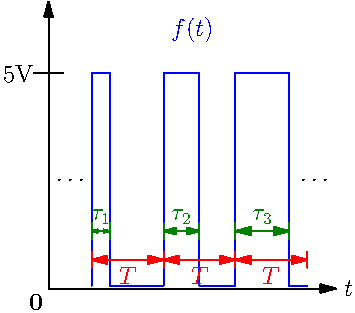
\includegraphics[width=2in]{pwm2}
\end{figure}

A \underline{pulse-width modulated} (PWM) signal \underline{encodes} a value 
into a pulse width $\tau$ of a signal with periodicity $T$.

\begin{block}{Express the value $v\overset{?}{=} f(\tau, T)$}
Write an equation to assign a value given $\tau$ and $T$.  What range of values 
does your formula assign?
\end{block}
\end{frame}


%\frame{\frametitle{Definitions}
%Noise is random changes to the signal due to physical properties of the sensor.
%All sensors are subject to noise.  Noise can only be quantified by statistics, 
%as its actual value $n(t)$ cannot be known.
%
%It is desirable for a control system to be \underline{Robust} to noise, 
%meaning 
%that the noise does not strongly affect the output.
%
%\underline{Uncertainty} is the incorrect (or absent) modeling of a system.
%}


\section{Sensors}
\subsection{Simple}
\frame{
\frametitle{Contact switch}
\begin{figure}
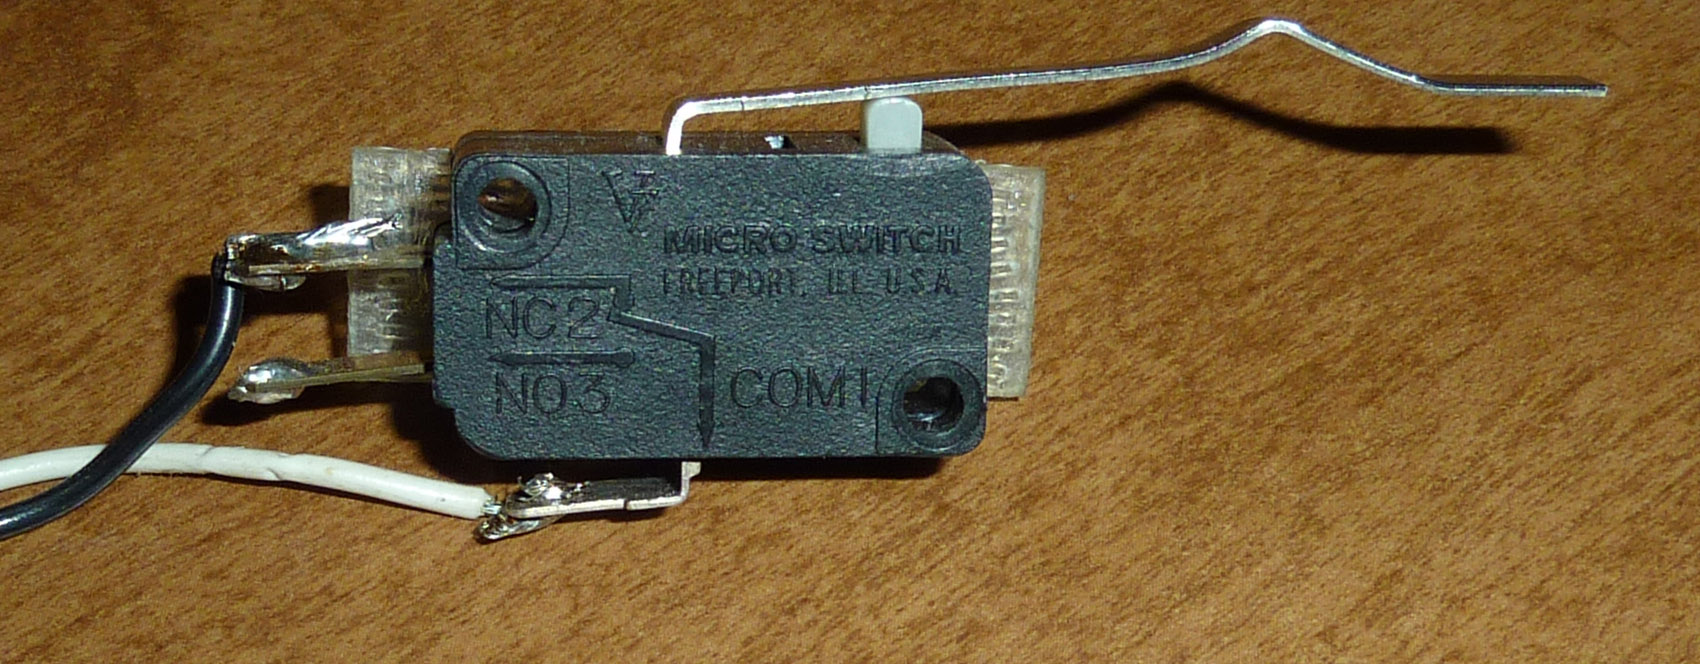
\includegraphics[width=2in]{LimitSwitch}
\end{figure}

We can treat this sensor like a digital signal.
\underline{Normally Open} (NO) is 0 at rest, 1 when pressed.  
\underline{Normally Closed} (NC) is 1 at rest, 0 when pressed.  Only need 2 
wires (ground and signal), because the \underline{Common} (COM) is connected to 
either NC or NO, but not both.

Difficulty: metal bends easily.
}

\frame{
\frametitle{Electronic switch}
\begin{figure}
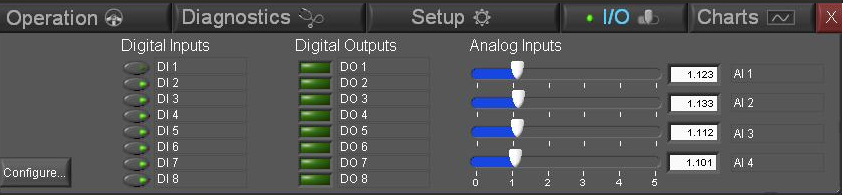
\includegraphics[width=\textwidth]{DriverStation}
\end{figure}

Available on the Driver Station program on the Laptop, these analog and digital 
are virtual hardware inputs to the robot.  The digital outputs are virtual LEDs 
on the robot.

The names of each can be changed by double clicking on the entry; the names are 
saved in a Driver station configuration file.

Difficulty: values can be set before a match, but not commonly changed during 
the match.
}

\frame{
\frametitle{Pressure switch}
\begin{figure}
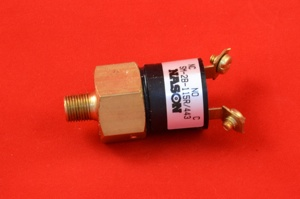
\includegraphics[width=2in]{PressureSwitch}
\end{figure}

We can treat this sensor like a digital signal and it only needs 2 
wires (ground and signal).

Must be installed for pneumatic system --- programming the \texttt{Compressor} 
class object requires the Digital input for this sensor.
}

\frame{
\frametitle{Potentiometer}
\begin{figure}
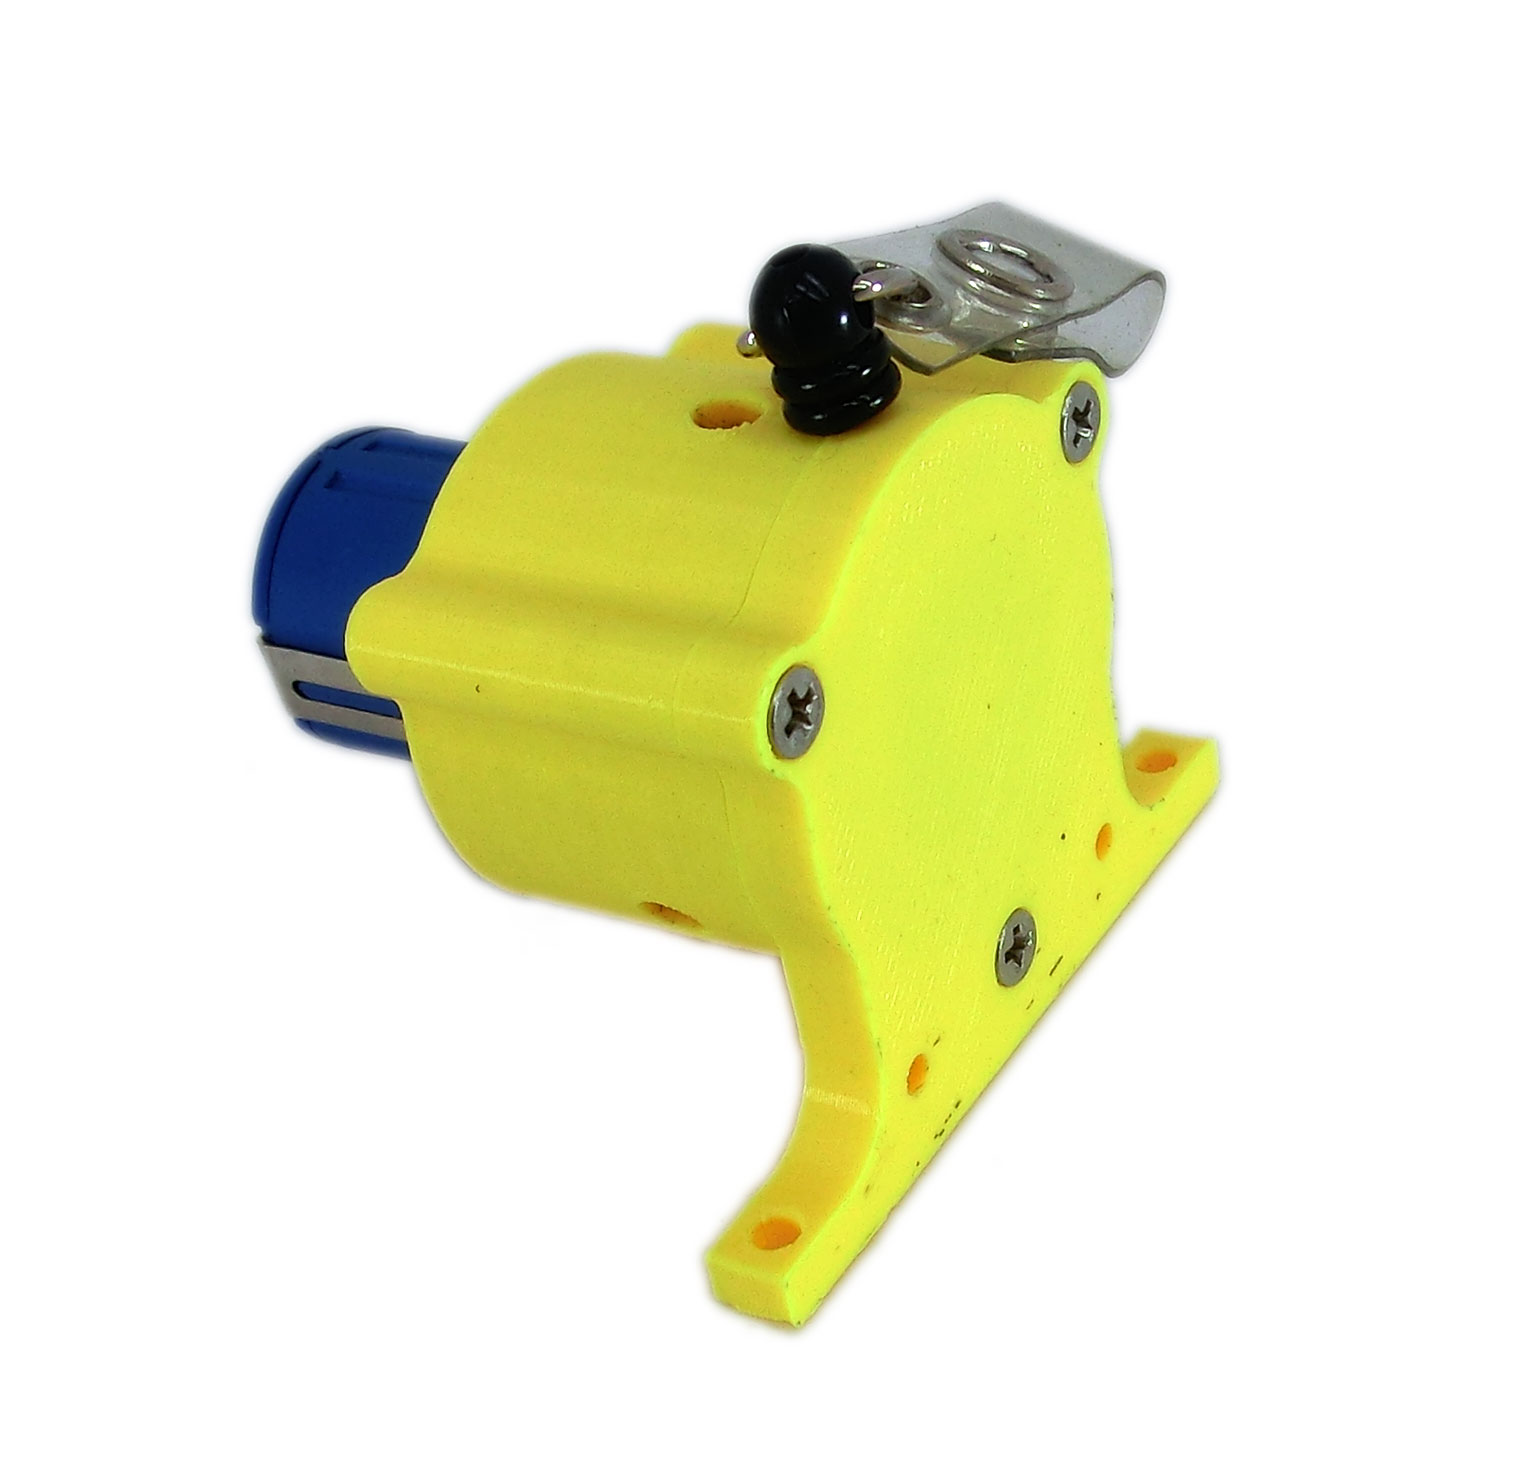
\includegraphics[width=1in]{Potentiometer}
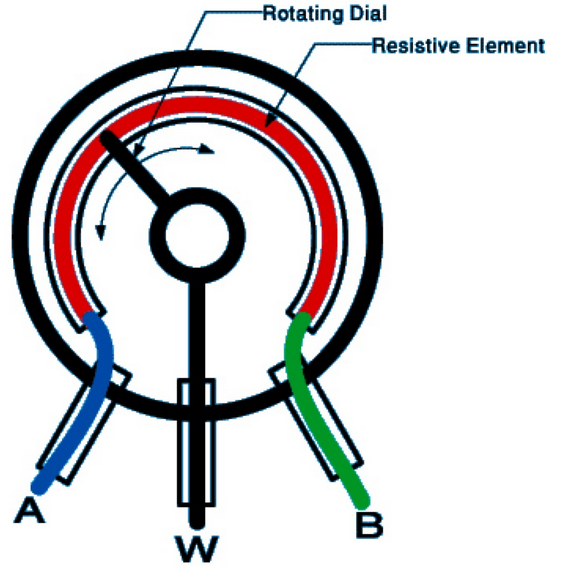
\includegraphics[width=1in]{Potentiometer2}
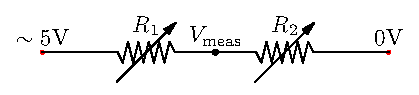
\includegraphics[width=2in]{resistors}
\end{figure}

Needs 3 wires, treated as an analog input.  This circuit is called a 
\underline{voltage divider} and it is modelled as two 
\underline{variable resistors} in \underline{series}.
\begin{equation*}
V_\text{meas}=\left(\sim 5 \text{V}\right) \times 
\left(\frac{R_2}{R_1+R_2}\right)
\text{where } R_1 + R_2 = \text{constant}
\end{equation*}

Pros: Fairly sensitive.  Cons: Does have a \underline{short circuit} position.
}

\begin{frame}[shrink]{Rotary encoder}
\begin{figure}[width=\textwidth]
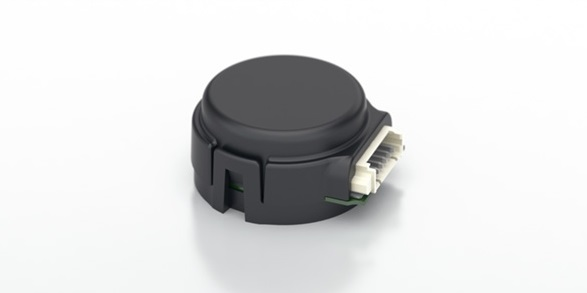
\includegraphics[width=1in]{OpticalEncoder}
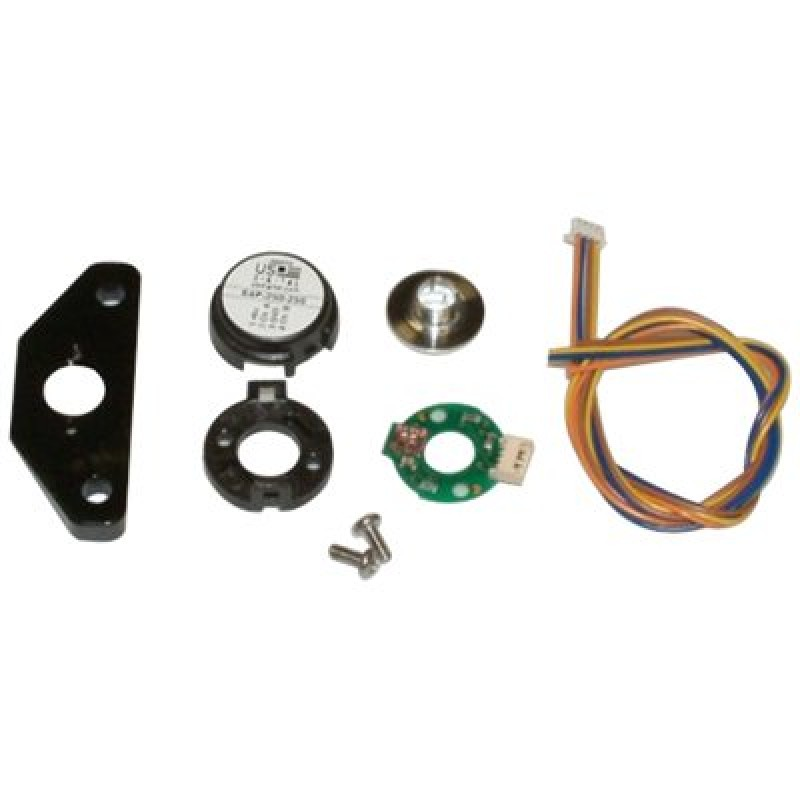
\includegraphics[width=1in]{OpticalEncoder2}
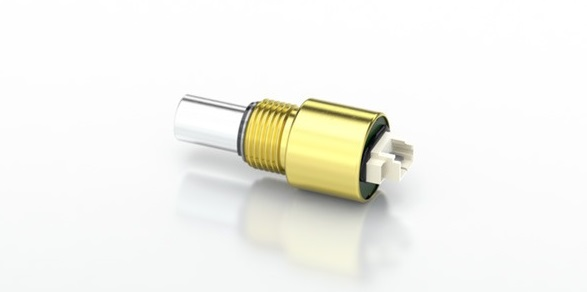
\includegraphics[width=1in]{MagneticEncoder}
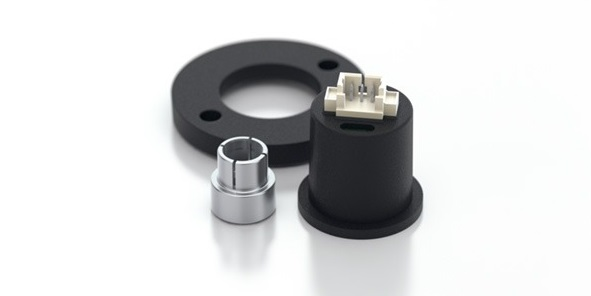
\includegraphics[width=1in]{MagneticEncoder2}
\caption{Left: Optical, Right: Magnetic}
\end{figure}

Uses 2 PWM signals in \underline{quadrature} that are connected to 2 digital 
inputs.  A single PWM signal would not contain rotation direction information, 
but using 2 PWM signals allows for direction to be known.

Difficulty: Optical sensor gets dirty with lazy handling (useless).  Plastic 
case clips break if the casing needs to be opened after closing.  Aligning the 
sensor to the rotating axle.  Small wires must be soldered to PWM cables 
to connect to digital inputs (messy wiring).
\end{frame}

\begin{frame}[shrink]{Rotary encoder}
\begin{figure}[width=\textwidth]
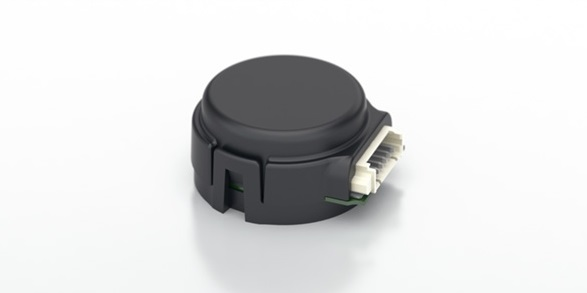
\includegraphics[width=1in]{OpticalEncoder}
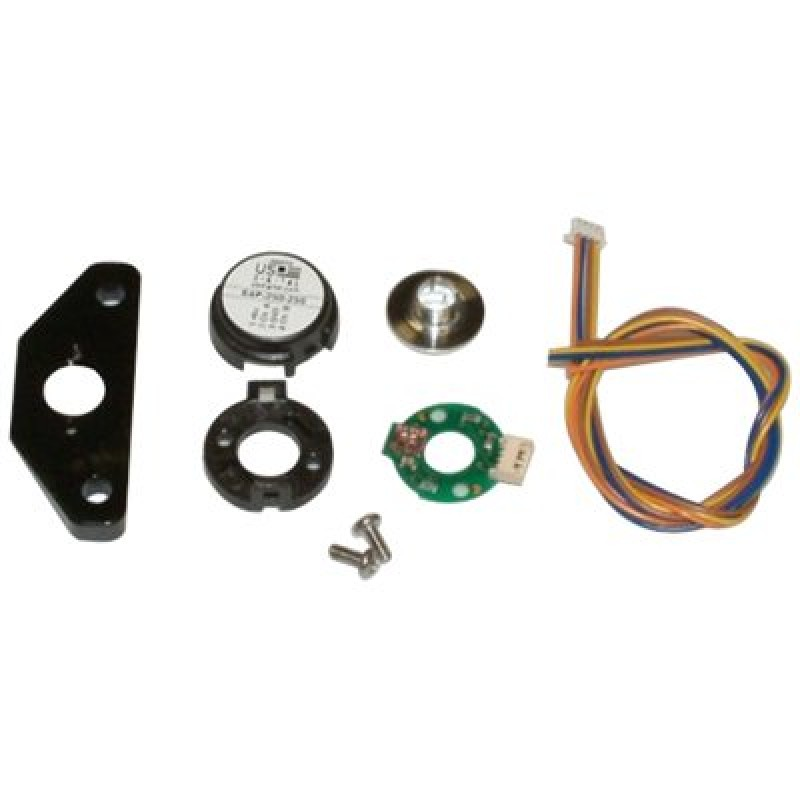
\includegraphics[width=1in]{OpticalEncoder2}
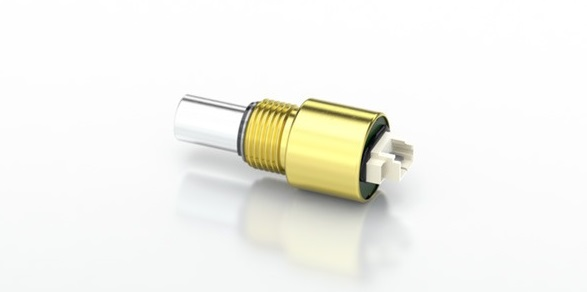
\includegraphics[width=1in]{MagneticEncoder}
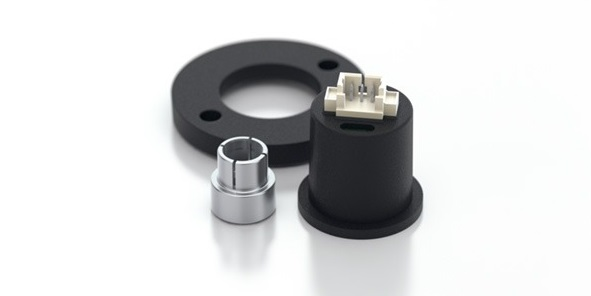
\includegraphics[width=1in]{MagneticEncoder2}
\caption{Left: Optical, Right: Magnetic}
\end{figure}

Uses: motor speed, distance estimation (\underline{trajectory following}), 
autonomous or 
\underline{fly-by-wire}.

One per side of robot? One per wheel? Separate free-spinning wheels?
\end{frame}

\subsection{Imaging}
\frame{
\frametitle{AXIS Webcam}
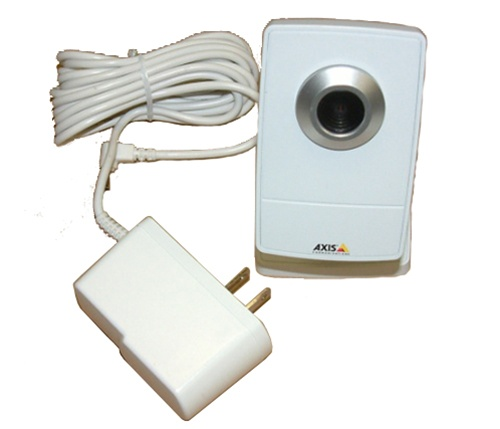
\includegraphics[width=1in]{AXISwebcam}

Traditional FRC hardware for a camera.  This camera plus a LED ring has been 
the basis for most FRC vision processing.
}

\frame{
\frametitle{PixyCam}
\begin{wrapfigure}{l}{1in}
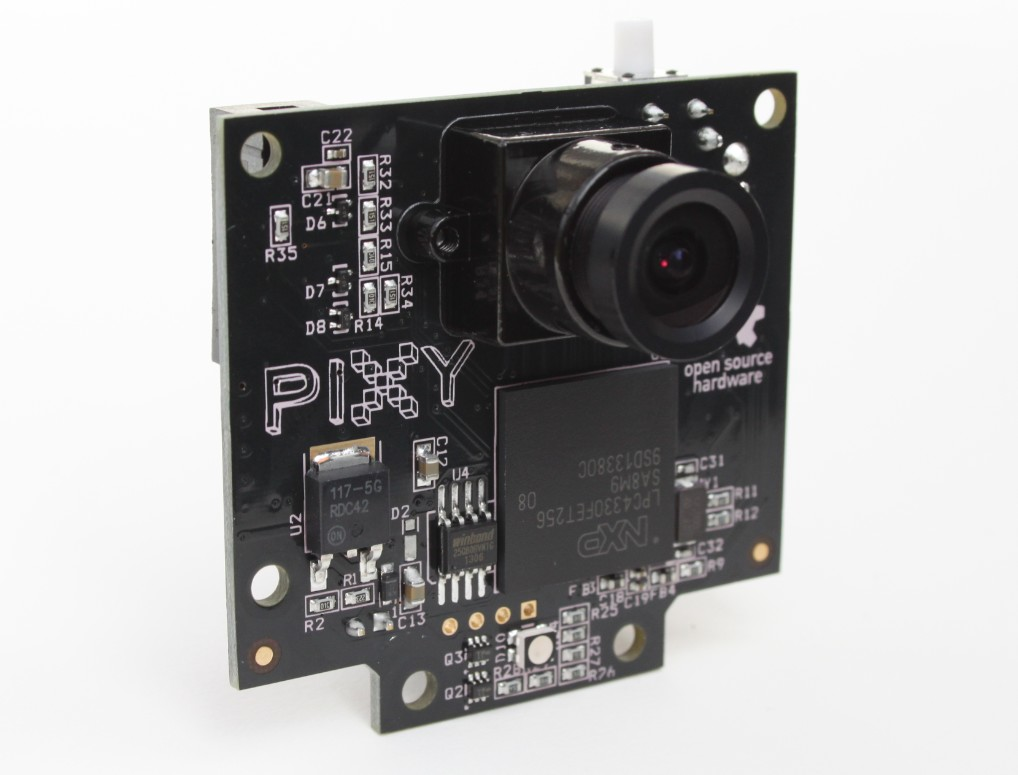
\includegraphics[width=1in]{PixyCam}
\end{wrapfigure}
These devices process the image on-board (inside the Pixy!) very quickly.  We 
could program the firmware to look for specific colored objects.  The camera 
connects easily to I2C, SPI, UART, digital outputs, several of which are on the 
RobotRIO.  These devices also connect easily to an arduino, and we could 
network the arduino to the RobotRIO.

I have 4 of these cameras and wanted to look into mounting multiple ones onto 
the robot.  We can also purchase servo kits to make the cameras move relative 
to the robot frame (they could search for objects without the robot base 
moving).
}

\frame{
\frametitle{Kinect}
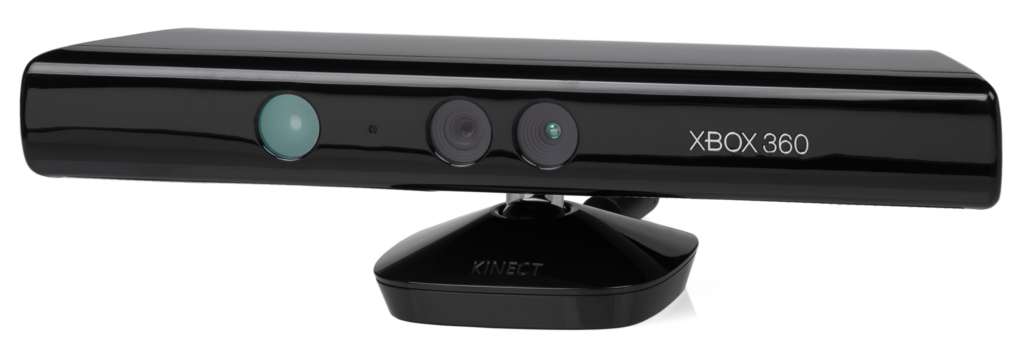
\includegraphics[width=1in]{kinect}

The Kinect is easy to hook up to a desktop computer, but perhaps the RobotRIO 
would support a direct connection since it now has USB.  The kinect provides a 
camera and depth (distance) information that we could use for a variety of 
purposes.
}

\frame{
\frametitle{Playstation Camera}
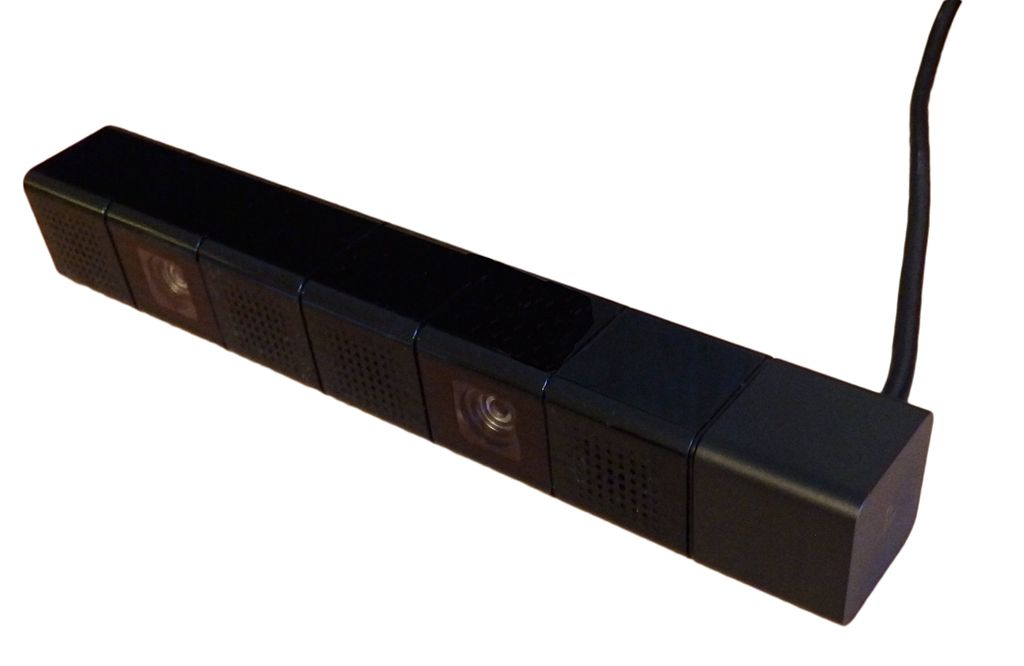
\includegraphics[width=1in]{PlaystationCamera}
Same as the kinect, need to investigate how easy it is to connect to the 
RobotRIO.
}

\subsection{Distance estimation}
\frame{
\frametitle{Ultrasonic rangefinder}
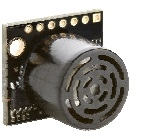
\includegraphics[width=1in]{Ultrasonic}
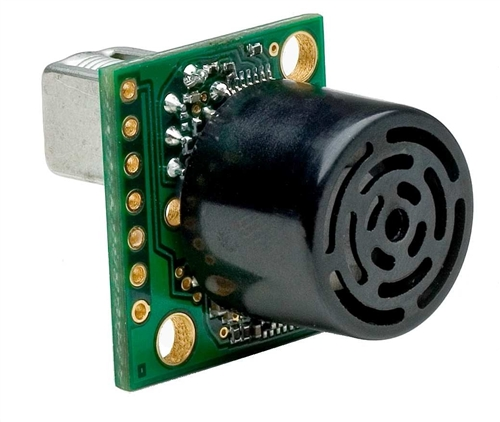
\includegraphics[width=1in]{Ultrasonic2}

The ultrasonic can measure a linear distance up to about 20 feet away.  
Mounting several of these on the robot could allow us to do a variety of 
control approaches (such as maintaining a particular distance to a target).

Cons: wiring can be tricky.
}

\frame{
\frametitle{Laser rangefinder}
\begin{figure}
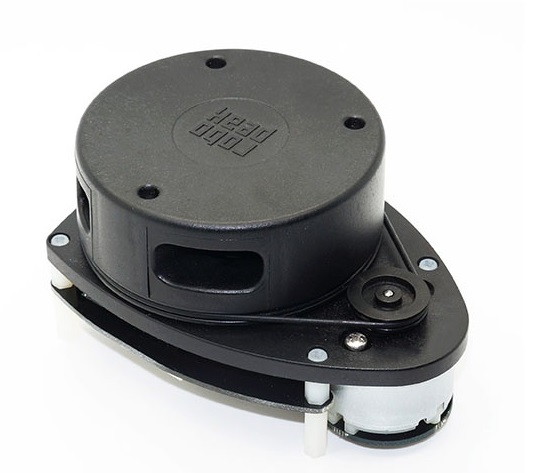
\includegraphics[width=1in]{LaserRangefinder}
\end{figure}

Unfortunately, lasers are not permitted by FRC rules.  But these are very 
powerful in robotics research.
}

\subsection{Location and Orientation}
\frame{
\frametitle{GPS}
Unfortunately not possible in the arenas due to weak signal.  The non-military 
signal also has such a large error ellipse that it is not useful to determine 
position inside of the playing field.
}

\begin{frame}[shrink]{Indoor GPS}

This would be a lot of fun, but FIRST would need to build the indoor GPS around 
the playing field (\emph{e.g.} the stars below).

\begin{figure}
\centering
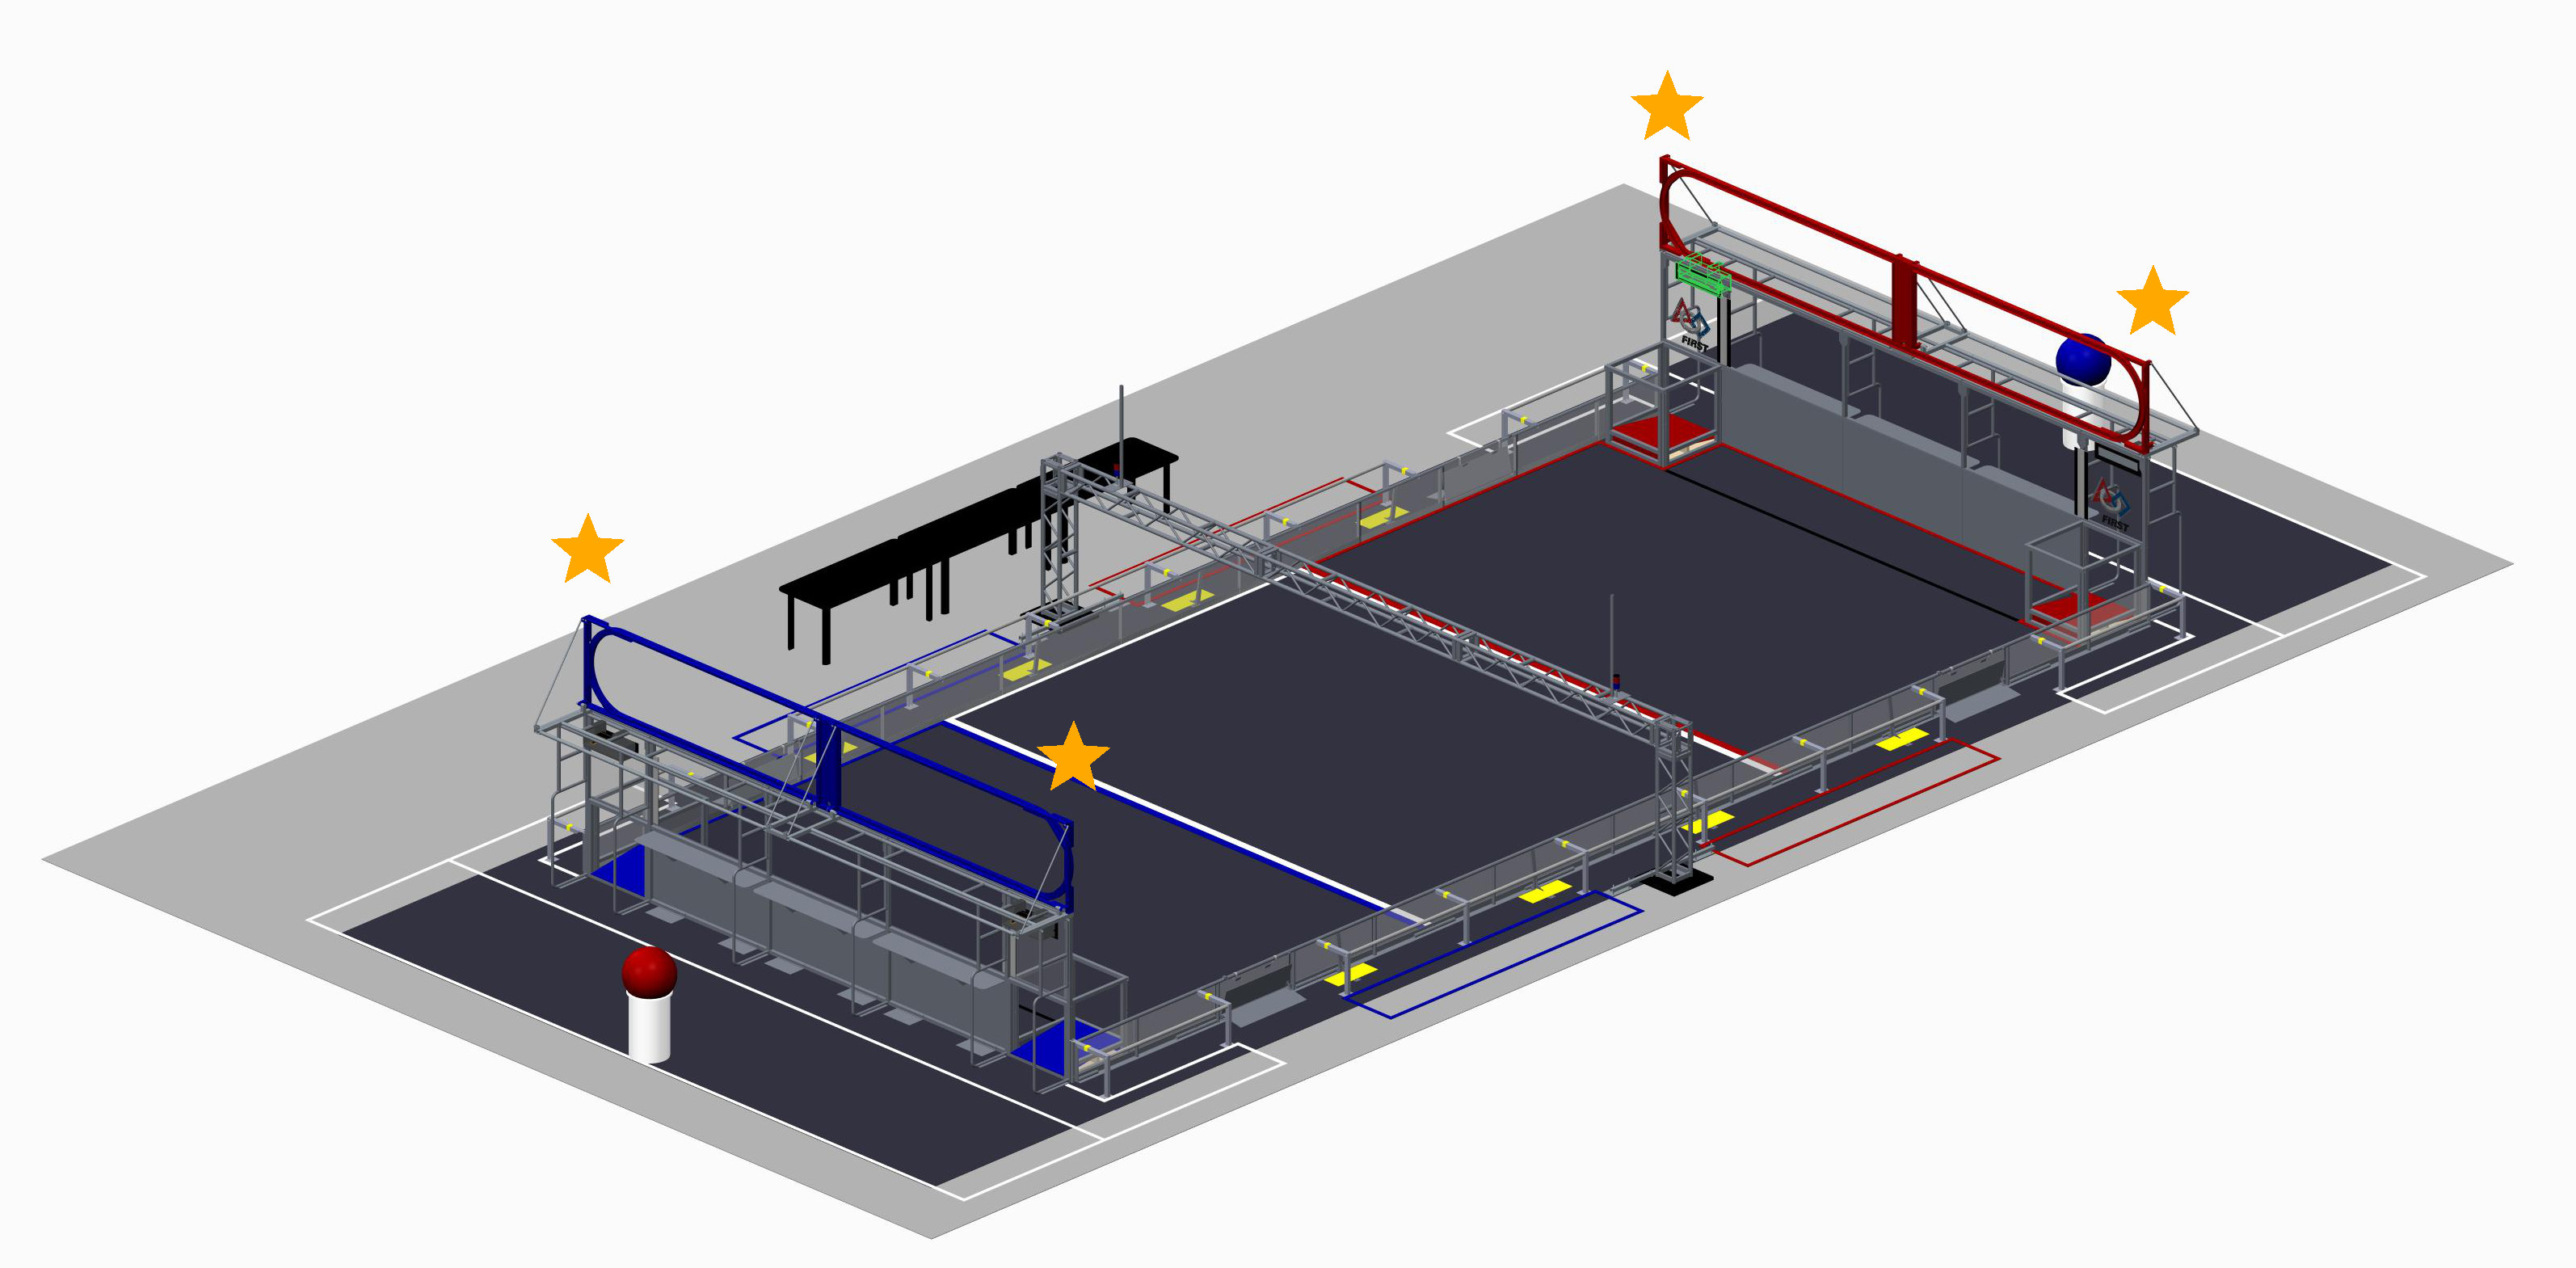
\includegraphics[width=\textwidth]{FRCarenaGPS}
\end{figure}

Would be novel if we use vision or other means to triangulate position on the 
field.
\end{frame}

\begin{frame}[shrink]{Trackball}
We could mount a trackball upside down on the robot.  The floor would cause the 
ball to roll.

\begin{figure}
\centering
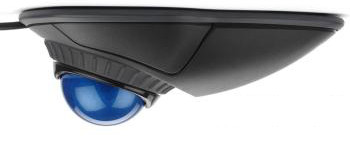
\includegraphics[width=\textwidth]{Trackball}
\end{figure}
This would be a lot of fun, but need to see if it would connect to RobotRIO.
Would be novel if we use it to estimate path on the field.
\end{frame}

\begin{frame}[shrink]{Occulus}

This would be a lot of fun, but need to see if we could do something with it.  
\begin{columns}
\begin{column}{0.5\textwidth}
\begin{figure}
\centering
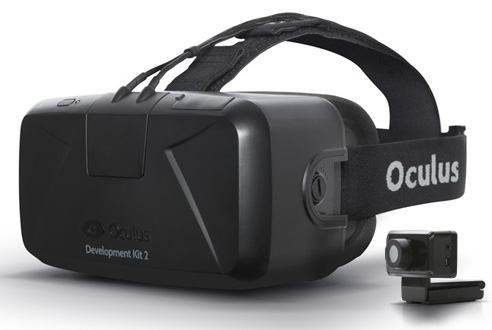
\includegraphics[width=0.9\textwidth]{Occulus}
\end{figure}
\end{column}
\begin{column}{0.5\textwidth}
\begin{itemize}
\item Move the robot based on human head rotation?  
\item Have a camera mounted on the robot with servos that looks where the human 
wants?
\item Human points a mechanism?  
\item Screen shows estimated projectile path 
overlayed camera view?
\end{itemize}
\end{column}
\end{columns}
\end{frame}

\frame{
\frametitle{Gyro}
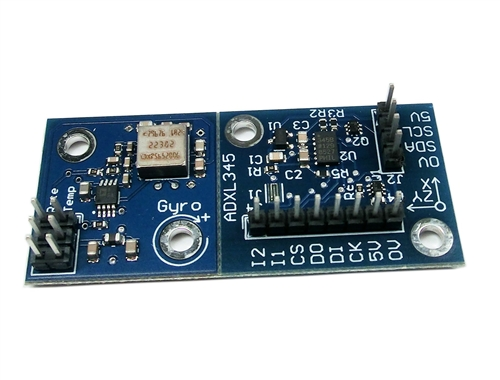
\includegraphics[width=1in]{Gyro}
}

\frame{
\frametitle{Accelerometer}
}





\section{Haptic and Controls}
\frame{
\frametitle{Vibrating joystick}
}

\frame{
\frametitle{Wii controller Wiimote}
}

\frame{
\frametitle{Wii balance board}
}

\frame{
\frametitle{LEGO Mindstorm}
The LEGO Mindstorm has equivalent sensors for:
color, light detection, axis rotation, contact, IR, ultrasonic, ...
}

\section{Conclusion}

\subsection{Resources}
\frame{ 
\frametitle{Resources}
[1] \href{http://www}{\underline{TBD}}
}

\end{document}
